\documentclass[12pt,a4paper,oneside]{report}%{article}% scrartcl

\usepackage[a4paper,left=1in, right=1in, top=1in, bottom=1in]{geometry}
\usepackage{graphicx} %% add [draft] for not generating figures (compiles much faster, in case only want to see text)
\usepackage{amsmath}
\usepackage{color}
\usepackage{colortbl}
\usepackage{tabularx} % voor zelf op te geven table breedte
\usepackage{multirow}
\usepackage[font={small,sf},labelfont=bf]{caption} 
\usepackage{hhline} % voor dubbele lijnen in een tabel
\usepackage{colortbl}
\usepackage{epsfig,subfigure}
\usepackage{natbib} %voor auteur-jaar citaties
%\usepackage[labelformat=empty]{caption} %% to remove the "Figure xx" from the figure and table captions
\usepackage{epstopdf} % when using pdflatex it changes eps figures into pdf so they can be included
\usepackage{pdfpages}
\usepackage{calc,keyval,ifpdf}
\usepackage[hidelinks]{hyperref}
\usepackage[xetex]{attachfile2} %% note to not put underscores in filenames and use only with pdf->latex
\usepackage{textcomp}
\attachfilesetup{color=0 0 1,print=true}
\usepackage[table]{xcolor}
\usepackage{pdflscape}
\usepackage[section]{placeins} %%  use \FloatBarrier command  to prevent floats to appear beyond some point in your document
\usepackage{threeparttable} % for footnotes in Tables
\usepackage{tabulary}
\usepackage{longtable} %% for tables spanning multiple pages
\usepackage[newcommands]{ragged2e}
\usepackage{booktabs} %% to use toprule bottomrule in table
\usepackage{array}
\newcolumntype{P}[1]{>{\centering\arraybackslash}p{#1}} %centering
%\newcolumntype{P}[1]{>{\RaggedRight\hspace{0pt}}p{#1}} %% use capital P in table to make them ragged right
\usepackage{soul}
\usepackage[parfill]{parskip} %changes the gap in front of paragraph
\setlength{\parindent}{0pt} %set indent = 0
\renewcommand{\baselinestretch}{1.5} %gap between lines
\graphicspath{ {Latex_images/} }

\begin{document}

\newpage

\begin{titlepage}

\newcommand{\HRule}{\rule{\linewidth}{0.5mm}} % Defines a new command for the horizontal lines, change thickness here

\center % Center everything on the page

%----------------------------------------------------------------------------------------
%	LOGO SECTION
%----------------------------------------------------------------------------------------

\includegraphics[width=0.5\linewidth]{aberdeen_logo}\\[1cm] % Include a department/university logo - this will require the graphicx package
 
%----------------------------------------------------------------------------------------
%	HEADING SECTIONS
%----------------------------------------------------------------------------------------

\textsc{\Large College of Physical Sciences}\\[0.5cm] % Major heading such as course name
\textsc{\Large School of Engineering}\\[0.5cm] % Major heading such as course name
\textsc{\Large $2^{nd}$ Year Report}\\[0.5cm] % Major heading such as course name

%----------------------------------------------------------------------------------------
%	TITLE SECTION
%----------------------------------------------------------------------------------------

\HRule \\[0.5cm]
{ \LARGE \bfseries Modelling and simulations of multiphase and multicomponent flows in porous media }\\[0.4cm] % Title of your document
\HRule \\[2.5cm]

%----------------------------------------------------------------------------------------
%	AUTHOR SECTION
%----------------------------------------------------------------------------------------

\begin{minipage}{0.4\textwidth}
\begin{flushleft} \large
\emph{Author:}\\
Konstantinos \textsc{Christou} % Your name
\end{flushleft}
\end{minipage}
~
\begin{minipage}{0.4\textwidth}
\begin{flushright} \large
\emph{Supervisors:} \\
Dr. Jefferson \textsc{Gomes}\\ % Supervisor's Name
Dr. Marcus C. \textsc{Bannerman}
\end{flushright}
\end{minipage}\\[7.5cm]

% If you don't want a supervisor, uncomment the two lines below and remove the section above
%\Large \emph{Author:}\\
%John \textsc{Smith}\\[3cm] % Your name

%----------------------------------------------------------------------------------------
%	DATE SECTION
%----------------------------------------------------------------------------------------

{\large \today}\\[3cm] % Date, change the \today to a set date if you want to be precise

%----------------------------------------------------------------------------------------

\vfill % Fill the rest of the page with whitespace

\end{titlepage}

\begin{center}
\section*{Abstract}
\end{center}
\addcontentsline{toc}{chapter}{Abstract}{}{}

In the current report the coupling between the multiphase and multicomponent flows is investigated. 
The motivation of this work is to model the coupled extended 3D Darcy equations with a compositional submodel. The resulting model will make use of a parametrised equation of state (EOS) to predict the PVT behaviour of light hydrocarbons and injection fluid in equilibrium. The result can be a new advanced reservoir simulator mainly for the
Oil \& Gas Upstream operations but not limited. 
The current work can be extended into EOR and CCS and carcon sequestrations operations, transport of contaminant in geological formations and in nuclear engineering applications.

The simulator is developed in two stages. The $1^{st}$ stage was the familiarisation with a set of computational tools for flow calculations to model most of the important characteristics of flow that occur in a porous media formations as well as investigate any flow instabilities that can occur. A number of cases (numerical simulations) has been undertaken in order to examine the development of flows in porous media. The $2^{nd}$ step is the development of a python scrypt to model the VLE/flash thermodynamics system. Currently we are at the stage of  code benchmarking. Experimental data for a $2$ component and $2$ phases system are used to compared with the numerical values that will result from the code.  

A model that can predict both multiphase flows and the distribution of chemical species, has many applications in the research area of geological multiphase-flows, range from fluid injection into geological formation to nuclear waste repository management, as well as water management.


\tableofcontents
\cleardoublepage
%\addcontentsline{toc}{chapter}{\listfigurename}
%\listoffigures
%\cleardoublepage
%\listoftables
%\addcontentsline{toc}{chapter}{\listtablename}
%\cleardoublepage

%\section{Motivation}
%In offshore engineering as well as large-diameter subsea pipelines, relatively small-diameter pipelines and cables are used to transport power and by-products and to control fluids for offshore operations. The stability of pipelines and cables on the seabed depends on hydrodynamic forces induced by waves and currents. For large waves in relatively shallow water, the forces are dominated by wave loading. Industry guidelines recommend that the wave forces are calculated based on "free-stream" flow properties, that is to say the properties of the flow near the bed as determined from an appropriate wave theory applied to the given wave and water depth conditions. Calculating free-stream flow ignores the presence of the wave boundary layer, which in reality, is always present. Determining wave loading based on free-stream flow, ignoring boundary layer effects, is sensible for conditions in which the diameter of the structure is large compared to the boundary layer thickness or when the cylinder is well away from the boundary. However, for relatively small diameter structures and relatively thick bottom boundary layers, which occur under long period waves, the structure may be wholly or substantially within the wave boundary layer. For such conditions, the wave loading will be determined by the boundary layer flow, not the free-stream flow.

\chapter{Introduction}

\section{Project background}

A number of problems of high interest in reservoir engineering involve multicomponent, two and three-phase flows in porous media. Species transfer between the phases affects the phase behavior and may change the phase densities and viscosities. Consequently flow instabilities will occur that can change the total behaviour of the system. In this work a conservative computational multi-fluid porous media flows model able to exploit mesh adaptivity methods on fully-unstructured tetrahedral grids is used. The model is based upon two key numerical characteristics: (a) a hybrid element-pair, \textit{$P_{n}DG-P_{m}DG$} family (b) the overlapping control volume finite element method (CVFEM) formulation. The $P_{n}DG-P_{m}DG$ element type offers discontinuous and piecewise representation for velocity and pressure fields at FE space while saturation and density scalar fields are calculated in control volume space \cite{Peksa2015237}. 

During the application of a 2-phase flow model each of the phases is considered to have a separately defined volume fraction (the sum of which is unity) and velocity field. Conservation equations for the flow of each species (with terms for interchange between the phases) can then be written down straightforwardly.

%The momentum equation for each phase is less straightforward. It can be shown that a common pressure field can be defined and that each phase is subject to the gradient of this field, weighted by its volume fraction. Transfer of momentum between the phases is sometimes less straightforward to determine, and, in addition, a very light phase in bubble form has a virtual mass associated with its acceleration. %(The virtual mass of a single bubble is about half its displaced mass).
The reason why multiphase flows are much more difficult to analyse than single phase flows is due to the fact of a large number of complex configurations. Practically for many cases, the homogeneous assumption is enough and suitable.

%However, this assumption will not be appropriate in other types of multiphase flows problems, so adopting this assumption might lead to a larger errors. 

%In oil and gas production, multiphase flow often occurs in wells and pipelines because the reservoirs produce gas and oil simultaneously. This is referred as two-phase flow. In addition to gas and oil, water is also often produced at the same time. This is called three-phase flow. Multiphase flows in porous media is an important part of the fluid mechanics and specifically of the Oil Industry since  60\% of the worlds' remaining oil reserves reside in fractured formations and there is a direct global energy \& economic interest.

IN addition, prediction of thermodynamic properties of natural reservoirs are important for both industrial and economic viewpoints.Equations of state (EOS) play an important role in the modelling of complex thermodynamic mixtures and they are the most common and convenient models for the study of phase equilibria of fluid multicomponent mixtures. 

There is an enormous amount of different EOS available for PVT and phase equilibria calculations. Cubic EOS have the ability to describe a VLE system and are widely used by the industry. Among many EOS the 2 most widely used in the oil and gas industry are the SRk-EOS and PR-EOS.  SRK-EOS fails to predict liquid dens
ities accurately. Improved density prediction was  the  main  motivation  of  the  authors  of  PR-EOS  which  in  general  is  superior  in  density predictions  of  reservoir  fluid  systems.  Although  this  equation  improves  the  liquid  density  
prediction,  it  cannot  describe  volumetric  behavior around  the  critical  point.  The  PR-EOS  is perhaps the most popular and widely used EOS $[5 , 6 , 10]$. 

\begin{figure}[h]
\center
\includegraphics[width=18. cm,height=10 cm]{./figures/Scheme-of-the-equation-of-state-EOS-study-proposed-in-this-work.png}
\caption{Scheme of the equations of state (EOS)}~\label{case1:simple_profile}
\end{figure}

%\section{Research aims and objectives}

%This project lies within areas of Oil \& Gas engineering (computational reservoir engineering, EOR), environmental science and technology (CCS, groundwater contaminat transport). 

%The aims of the project is to develop an advanced computational methods for multi-fluid compositional flows in porous media. The new model approach will significantly improve our ability to predict the behaviour of light hydrocarbons through geological porous media.

%The current simulator is intentioned to be general in its applicability, such that other industrial or environmental problems can be simulated. The aim of the present work is to try to bring much of this fundamental understanding together into one report %fig.\ref{fig:Method_Disciplines} 
%and to present a unifying approach to the fundamental ideas of multiphase and reactive flows flows. In order to perform the future simulations related with the project, we will develop our own simulator for multiphase flow in porous media, which will couple reactive transport of chemical species and transport equations all based in one specific open source software called, \textit{Fluidity}.

\chapter{The Model}

%\section{Model Formulation}
The model will be based on the multiphase and multicomponent formulations as these are expressed by the equations below. 

The Multiphase flow is expressed by the darcy's equation and the saturation eq. using the control volume finite element method (CVFEM).The multicomponent part is described by the modifies Peng-Robinson equation of state (EOS). 

In this case, a stochastic method is used to describe the flash system (VLE). This method will give us a relation between the minima of gibbs free energy and the composition of species in our system. We choose the \textcolor{red}{smallest, of the least of the minima} that describes the minimum gibbs energy of our system. For this minimum a pair of composition of species can be found. This pair will define the equilibrium composition of our system.  
 
\section{Multiphase Flow}

Each discontinuous phase from the microscopic level is replaced by a continuum on the macroscopic level. We suppose that the void space contains -m- fluid phases either denoted by Greek symbols $\alpha$ or $\beta$, or Latin symbols, w, n, g.

\textit{Conservation of Mass}. Suppose that the porous medium fills the domain $\Omega \subseteq \Re^3$. Then the conservation of mass for  each phase $\alpha$ is given by the Eq. \ref{eq: 2.2.9}.  

\begin{equation}
 \frac{\partial( \Phi \rho_a S_a)}{\partial t} + \nabla \cdot \{\rho_a u_a S_a\} = \rho_a q_a 
\label{eq: 2.2.9}
\end{equation}  

\noindent or it can be rewritten in the form of saturation equation, for incompressible flow when $\rho$ is constant, as follows (Eq. \ref{eq: 2.2.10}), 

\begin{equation}
\Phi \frac{\partial(S_a)}{\partial t} + \nabla \cdot \{u_a S_a \} = S_{cty,a} 
\label{eq: 2.2.10}
\end{equation}  

\noindent Each phase has its own density, $\rho_a$, saturation $S_a$, velocity $u_a$ and source term $q_a$.
\textit{Extension to Darcy 's Law}. As in the single-phase case it can been shown by volume averaging or homogenization techniques that the macroscopic phase velocity can be described as a function of phase pressure as,

\begin{equation}
u_a = - \frac{K_a}{\mu_a} \cdot (\nabla p_a - \rho_a g)
\label{eq: Darcy's law}
\end{equation}  

In addition to the assumptions in the single-phase case it has been assumed that the momentum transfer between phases is negligible. The phase permeability $K_a$ , however, depends on the saturation of phase $\alpha$ and can be further decomposed into

\begin{equation}
K_a= K_{ra} (S_a) K
\label{eq: 2.2.12}
\end{equation}

\noindent i.e. scalar non-dimensional factor $\kappa_{ra}$ is called \textit{relative permeability} and the absolute permeability \textit{K} which is depended of the fluid. Eq.\ref{eq: 2.2.9} is due to (Muskat et al. 1937). The relative permeability $\kappa_{ra}$, models the fact that the flow paths of fluid $\alpha$ are blocked by the presence of other phases. This scaling factor follows the constraint below,

\begin{equation}
0 \le k_{ra} (S_a) \le 1.
\label{eq: 2.2.13}
\end{equation} 

By using the \ref{eq: 2.2.8} \& \ref{eq: 2.2.9} equations, we obtain the final form of \textit{Darcy 's Law for Multiphase Flows} that will be used later in the solution that we try to develop.

\begin{equation}
u_a = - \frac{k_{ra}}{\mu_a} \cdot K \cdot (\nabla p_a - \rho_a g)
\label{eq: 2.2.14}
\end{equation}

\noindent while the quantity, $\lambda_a = - \frac{k_{ra}}{\mu_a} $ is often referred as \textit{mobility}.
 
 
\subsection{Flow Instabilities} 

\textit{Viscous fingering} is a viscous driven hydrodynamic instability that results the collapse of the uniform interface between the fluids of different viscosity. The mechanisms that govern this phenomenon are,  \textit{shielding}, \textit{spreading} and \textit{tip-splitting}. Tip-splitting, fig.\ref{fig:tip}, happens when a finger becomes unstable and splits into two branches. These can be found mainly in porous medium when the flow velocity is not large. 

%\begin{equation}
%Pe = \frac{Advective\;transport\;rate}{diffusive\;transport\;rate} 
%\label{eq: Pe}
%\end{equation}

%\begin{equation}
%Mobility\;Ratio = \frac{\mu\;of\;the\;injected\;fluid}%{\mu\;of\;the\;displaced} 
%\label{eq: MR}
%\end{equation}

%\begin{figure}[!h]
%\centering
%\begin{minipage}[!h]{0.45\linewidth}
%\center{\includegraphics[width=1.1\linewidth]{figures/tip-splitting}}
%\caption{Tip-splitting in viscous fingering}
%\label{fig:tip}
%\end{minipage}
%\hfill
%\begin{minipage}[!h]{0.45\linewidth}
%\center{\includegraphics[width=1.1\linewidth]{figures/shielding}}
%\caption{Shielding in viscous fingering}
%\label{fig:shielding}
%\end{minipage}
%\end{figure}


%Viscous fingering has been found to influence industrial processes such as the removal of oil from reservoirs, the potential use of $CO_2$ sequestration and the re-mediation of spills, or the transport of pollutants in aquifers. Viscous fingering  is highly related with the mobility, which describes how easily a fluid moves into a porous media and can be expressed through the mobility ratio (Eq.\ref{eq: MR}).The primary removal of oil from reservoirs leaves the porous reservoirs with remaining oil that can only be removed by the use of enhanced oil-recovery (EOR). This secondary and tertiary removal of oil from porous beds is required to be as efficient and economically viable as possible.
 
Regarding the viscous fingering mechanics, lets assume a porous medium, characterized by a constant permeability $K$. The flow will typically involve the displacement of a fluid of viscosity $\mu_1$  and density $\rho_1$ by a second fluid of viscosity $\mu_2$ and density $\rho_2$. Under suitable continuum assumptions,\textit{Darcy's law}  is used to describe the flow through a porous medium.

\begin{equation}
 U = \frac{b^2}{12 \mu} \nabla p
\end{equation}

and the above equation can be re-arranged for 1D steady flow as,

\begin{equation}
 \frac{dp}{dx}= - \frac{\mu U}{K} + \rho g 
\end{equation}

where, \textit{U}, is the velocity of the more viscous fluid, \textit{b}, is the cell gap (referring to Hele-Shaw cell) and \textit{$\nabla p$} is the pressure gradient.



Now consider a sharp interface or zone where density, viscosity, and solute concentration all change rapidly. Then the pressure force 
$(p_2 - p_1)$ on the displaced fluid as a result of a virtual displacement $\delta_x$ of the interface from its simple convected location is 

\begin{equation}
\delta p=(p_2-p_1)= \left[\frac{(\mu_1-\mu_2)U}{K}]+(\rho_2-\rho_1)g \right] \delta x
\end{equation}

If the net pressure force is positive, then any small displacement will amplify, leading to an instability.In this case gravity is a stabilizing force while viscosity is destabilizing leading to critical velocity $U_c$ above which there is an instability.

\begin{equation}
U_c = \frac{(\rho_1-\rho_2) \cdot g \cdot K}{(\mu_1-\mu_2)}
\end{equation} 

\subsection{CVFEM formulation}

For porous media flows, CVFEM discretisation with Galerkin-FEM formulations for pressure equation has been used to solve the Darcy \& Richard equations. In order to approach and set up the $1^{st}$ part of this project a novel finite element method formulation to solve subsurface multi-fluid flows will be introduced. It is described as the overlapping control volume finite element method, \textit{OCVFEM}. %This formulation has two major advantages, since it is a dual consistent pressure-velocity representation in control volume and finite element spaces which ensure local mass balance. It uses recently developed family of finite element types that ensure that the Darcy's equation for multiphase flows are exactly applied in 1D. 

The mass conservation equations are solved in control volume space and finite elements are used in order to obtain the high-order fluxes on the control volume boundaries. The continuity equations are embedded into the pressure equation to enforce mass and force balance. 

%We imply an implicit algorithm with respect to time. 

Regarding the \textit{$P_n DG -P_{n+1}$} element type that is going to be applied, it is a dual consistent pressure-velocity representation of CV \& FEM spaces into a triangular and tetrahedral finite element pairs. The \textit{$P_1 DG -P_2$} element was developed to represent the balance of geostrophic pressure and velocity without introducing spurious pressure nodes.Fig.\ref{fig:element type} below displays the three types of the \textit{$P_n DG -P_{n+1}$} family.

%\begin{figure}[!h]
%\begin{minipage}{0.5\linewidth}
%\center {\includegraphics[clip,width=1\textwidth]{figures/p0dgp1-cont-sat}\\a)}
%\end{minipage}  
% \hfill 
%\begin{minipage}{0.5\linewidth}
%\center {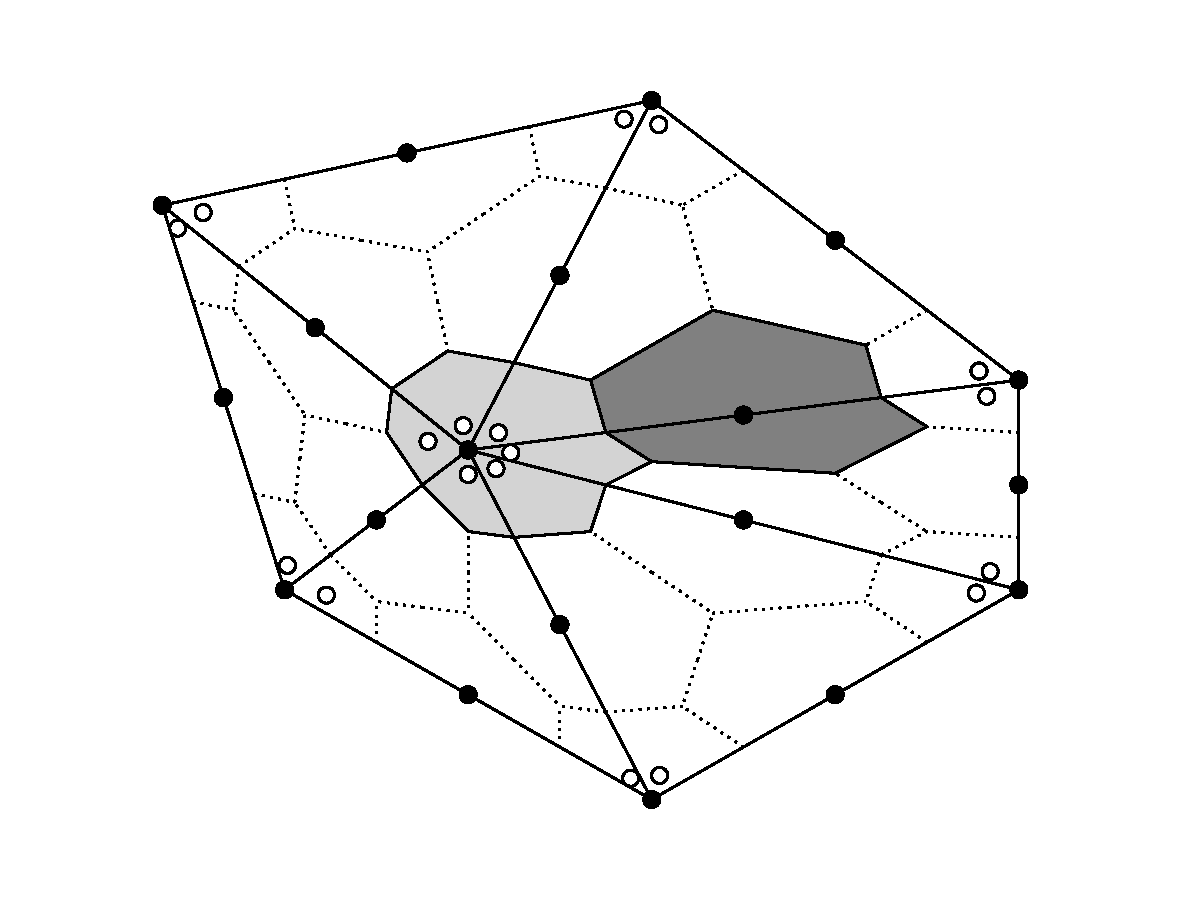
\includegraphics[clip,width=1\textwidth]{figures/p1dgp2-cont-sat}\\b)}
%\end{minipage}  
%\hfill
%\center 
%\begin{minipage}{0.65\linewidth}
%\center {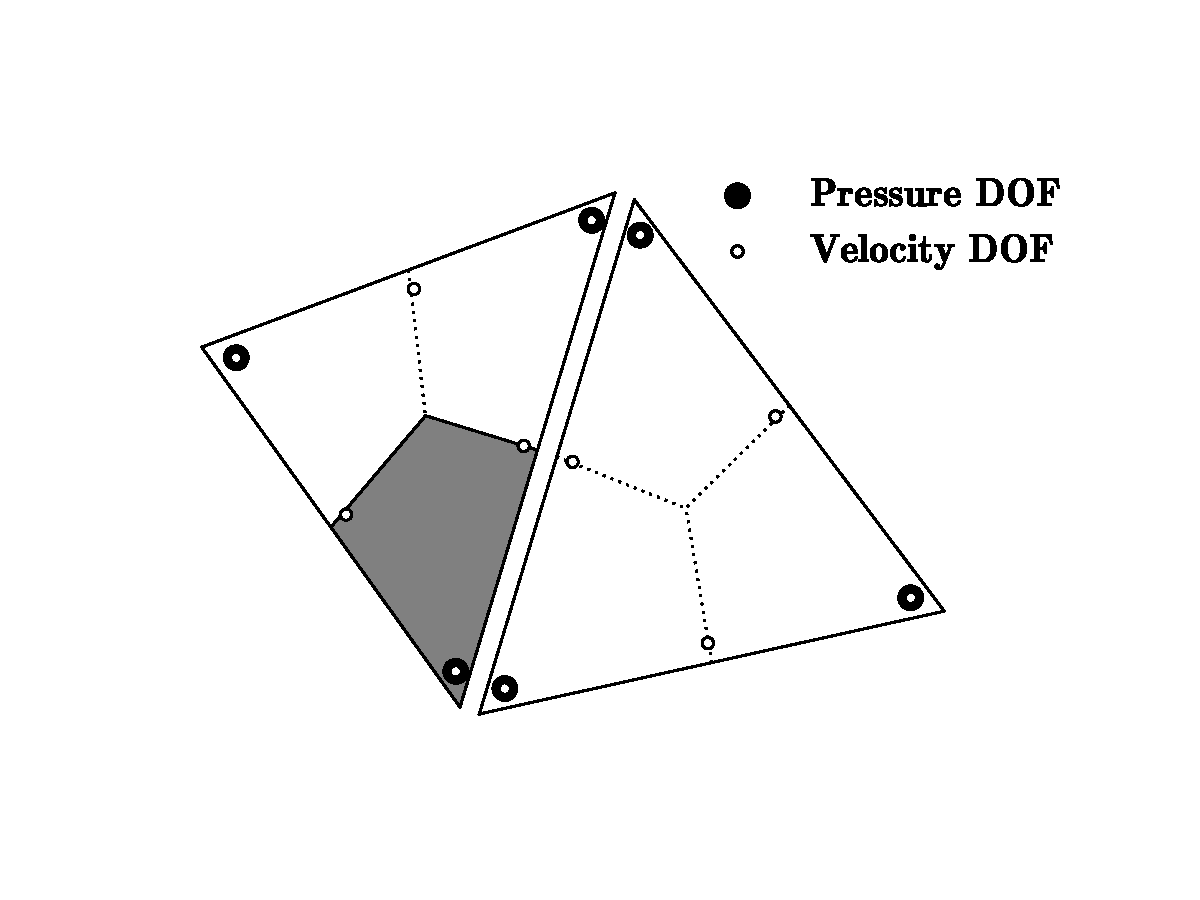
\includegraphics[clip,width=1\textwidth]{figures/p2dgp1-dg-sat}\\c)}
%\end{minipage}

%\caption{\label{fig:element type} (a) $P_0 DGP_1$, (b) $P_1DG P_2$, (c) $P_2 DGP_1$, Shaded areas denote a control volume (in which saturation is stored), black points represent the pressure nodes and white points the velocity}
%\end{figure}

%Defining this element type above, the dual velocity and pressure fields are represented by the $n^{th}$  -(discontinuous) and $(n+1)^{th}$ -order (continuous) polynomials respectively. This allows the velocity to exactly represent pressure gradient in the solution for homogeneous material properties. The extension of \textit{$P_n DG P_{n+1}$} is the \textit{$P_{n+1} DG -P_n DG$} element that has similar properties but allows a fully discontinuous representation of pressure, saturation and other quantities between the elements.

\subsubsection{Overlapping-CVFEM Formulation}

Darcy's law for immiscible multiphase flows may be written as:

\begin{equation}
q_a = - \frac{K_{ra} S_a \textbf{K}}{\mu_a} (\nabla p_a - S_{ua})
\label{eq: darcy}
\end{equation}

\noindent where $q_a = (q^{(1)}_a, q^{(2)}_a,q^{(3)}_a)$, fro $3D$ flow is $a-th$ phase Darcy flow rate, \textbf{K} is the absolute permeability tensor, $K_{ra} (S_a)$ is the phase relative permeability and is a function of the phase saturation $S_a(r,t)$ and $\mu_a$, $p_a$ and $s_{ua}$ are the phase dynamic viscosity, pressure and a source term respectively.
 
 If we define the advective velocity averaged over the entire medium as $u_a= \frac{q_a}{S_a}$ then we can rewrite the the above eq. \ref{eq: darcy} as, 
 
\begin{equation}
\underline{\underline{\sigma_a}} u_a = \ \nabla p + s_{ua}
\label{eq: 2.4.2}
\end{equation}   

\noindent where  $\underline{\underline{\sigma_a}} = \mu_a S_a {(K_{ra} \textbf{K})^{-1}}$ represents the implicit linearisation of the viscous frictional forces. To discretise the Eq.\ref{eq: 2.4.2}, we assume a finite element representation for the velocity and the pressure fields and a control volume representation for phase saturation fields. This can be represented as, 

\begin{equation}
M_{\sigma} \underline{u} = -C \underline{p} + {\underline{s}_u}
\end{equation} 

\noindent where ($\underline{u}$) is the phase velocity and ($\underline{p}$) solution vectors.  

\pagebreak

\section{Multicomponent system}

\subsection{Mass Balance}
For a system with $n_{p}$ phases and $n_{c}$ components, the mass of each phase $j$ is,
\begin{equation}
m^{j} = \summation_{i=1}^{n_{c}}m_{i}^{j}\;\;\;\text{ for }j=1,2,\cdots,n_{p}
\label{Eqn_MassBalance_Phase}
\end{equation}

And the mass of each component $i\left(=1,2,\cdots,n_{c}\right)$,
\begin{equation}
m_{i} = m_{i}^{1} + m_{i}^{2} + \cdots + m_{i}^{n_{p}} = \summation_{j=1}^{n_{p}}m_{i}^{j}
\label{Eqn_MassBalance_Component}
\end{equation}

The total mass $m$ can be define as,
\begin{equation}
m - m^{1} + m^{2} + \cdots + m^{n_{p}} = \summation_{j=1}^{n_{p}}m^{j} = \summation_{i=1}^{n_{c}}m_{i}
\label{Eqn_MassBalance_Mass}
\end{equation}

Defining the intensive properties:
\begin{eqnarray}
w_{i}^{j} = \frc{m_{i}^{j}}{m^{j}} \label{Eqn_MassBalance_MassFraction} \\
z_{i} = \frc{m_{i}}{m} \label{Eqn_MassBalance_MassFractionFeeding} \\
\Pi^{j} = \frc{m^{j}}{m}\label{Eqn_MassBalance_PhaseMassFraction} 
\end{eqnarray}
where $w_{i}^{j}$ is the mass fraction of component $i$ in phase $j$, $\Pi^{j}$ is the mass fraction of phase $j$ and $z_{i}$ is the overall feed mass fraction of component $i$. 
%From Eqns.~\ref{Eqn_MassBalance_Mass}-~\ref{Eqn_MassBalance_PhaseMassFraction}, we can define normalised quantities, i.e., fractions, and we can add the following constraints:
%\begin{eqnarray}
%&&w_{n_{c}}^{j} = 1 - \summation_{i=1}^{n_{c}-1}w_{i}^{j}  %\hspace{3cm} j=1,2,\cdots,n_{p}  %\label{Eqn_MassBalance_MassFraction2} \\
%&&z_{n_{c}} = 1 - \summation_{i=1}^{n_{c}-1}z_{1}  \\
%&&\Pi^{n_{p}} = 1 - \left(\Pi^{1} + \Pi^{2} + \cdots + %\Pi^{n_{p}-1}\right) = 1 - \summation_{j=1}^{n_{p}-1} %\Pi^{j}\label{Eqn_MassBalance_PhaseMassFraction2}
%\end{eqnarray} 
%with
%\begin{displaymath}
%  z_{i} = \frc{m_{i}}{m} = %\frc{\summation_{j=1}^{n_{p}}m_{i}^{j}}%{m} \frc{m^{j}}{m^{j}} = %\underbrace{\frc{m^{j}}{m}}_{\red{\Pi^{j}}} \cdot %\overbrace{\frc{\summation_{j=1}^{n_{p}}m_{i}^{j}}%{m^{j}}}^{\red{\summation_{j=1}^{n_{p}}w_{i}^{j}}} 
%\end{displaymath}
%leading to
%\begin{equation}
%z_{i} = \Pi^{1}w_{i}^{1} + \Pi^{2}w_{i}^{2} + \cdots + %\Pi^{n_{p}}w_{i}^{n_{p}}
%\label{Eqn_MassBalance_FeedMassFractionConstraint}
%\end{equation}
%with
%\begin{equation}
%0\leq\Pi^{j}\leq 1 \hspace{3cm} 0\leq w_{i}^{j}\leq 1
%\end{equation}

If the solution is contained within \red{$n_{p}$} phases, the inequality can be rewritten as,
\begin{equation}
0 < \Pi^{j} < 1
\end{equation}
%Thus 
%\begin{displaymath}
%\Pi^{k} = 1 - \summation_{j=1,j\neq k}^{n_{p}} \Pi^{j} \neq 0
%\end{displaymath}
%Therefore from %Eqn.~\ref{Eqn_MassBalance_FeedMassFractionConstraint},
%\begin{equation}
%w_{i}^{k} = \frc{z_{i}+\summation_{j=1,j\neq %k}^{n_{p}}\Pi^{j}w_{i}^{j}}{\Pi^{k}} = \frc{z_{i} + %\summation_{j=1,j\neq %k}^{n_{p}}\Pi^{j}w_{i}^{j}}%{1-\summation_{j=1,j\neq %k}^{n_{p}}\Pi^{j}}
%\label{Eqn_MassBalance_FeedMassFractionConstraint2}
%\end{equation}



%\begin{mdframed}[style=JFrame]
For 2 phases, $\Pi^{1}=L$ and $\Pi^{2}=V$, the system becomes %Eqn.~\ref{Eqn_MassBalance_FeedMassFractionConstraint} becomes:
\begin{displaymath}
w_{i}^{V} = \frc{z_{i}-Lw_{i}^{L}}{1-L}
\end{displaymath}
for $i=1,2,\cdots,n_{c}$, and for 3 phases,$\Pi^{1}=L$, $\Pi^{2}=V$ and $\Pi^{3}=H$:
\begin{displaymath}
w_{i}^{H} = \frc{z_{i}-\left(V w_{i}^{V} + L w_{i}^{L}\right)}{1 - \left(V w_{i}^{V} + L w_{i}^{L}\right)}
\end{displaymath}
%\end{mdframed}

%% SUB-SECTION
\subsection{Free Gibbs Energy}
In thermodynamics, the Gibbs free energy (IUPAC recommended name: Gibbs energy or Gibbs function; also known as free enthalpy to distinguish it from Helmholtz free energy) is a thermodynamic potential that measures the maximum or reversible work that may be performed by a thermodynamic system at a constant temperature and pressure (isothermal, isobaric).The Gibbs energy (also referred to as G) is also the thermodynamic potential that is minimized when a system reaches chemical equilibrium at constant pressure and temperature. For equilibrium problems (e.g., vapour-liquid equilibrium, VLE), the total free Gibbs energy can be expressed as,
\begin{equation}
G = \summation_{j=1}^{n_{p}}\left(\summation_{i=1}^{n_{c}} m_{i}^{j}\mu_{i}^{j}\right)
\label{MassGibbs_Definition}
\end{equation} 
this represents
\begin{displaymath}
G = \summation_{i=1}^{n_{c}} m_{i}^{1}\mu_{i}^{1} + \summation_{i=1}^{n_{c}} m_{i}^{2}\mu_{i}^{2} + \cdots + \summation_{i=1}^{n_{c}} m_{i}^{n_{p}}\mu_{i}^{n_{p}}
\end{displaymath}
The chemical potential $\left(\mu\right)$ can be written as a function of the mass of each component at each phase,
%\begin{eqnarray}
%\mu_{i}^{j} &=& \mu_{i}^{j}\left(m_{1}^{j}, m_{2}^{j}, \cdots, %m_{n_{c}}^{j}\right) = \mu_{i}^{j}\left(\frc{m_{1}^{j}}{m^{j}}, \frc{m_{2}^{j}}{m^{j}}, \cdots, \frc{m_{n_{c}}^{j}}{m^{j}}\right)\nonumber \\
% &=& \mu_{i}^{j}\left(w_{1}^{j}, w_{2}^{j}, \cdots, w_{n_{c}}^{j}\right)\label{chempotential_functional}
%\end{eqnarray}
%Dividing Eqn.~\ref{MassGibbs_Definition} by $m$,
%\begin{equation}
%g = \frc{G}{m} = \summation_{j=1}^{n_{p}}\left(\summation_{i=1}^{n_{c}}\frc{m_{i}^{j}}{m}\mu_{i}^{j}\right) = \summation_{i=1}^{n_{c}}\frc{m_{i}^{1}}{m^{1}} \cdot \frc{m^{1}}{m} \mu_{i}^{1} + \cdots + \summation_{i=1}^{n_{c}}\frc{m_{i}^{n_{p}}}{m^{n_{p}}} \cdot \frc{m^{n_{p}}}{m} \mu_{i}^{n_{p}}
%\label{MassGibbs_Definition2}
%\end{equation}
%And we rewrite Eqn.~\ref{MassGibbs_Definition2} as,
%\begin{equation}
%g = \summation_{i=1}^{n_{c}}\Pi^{1}w_{i}^{1}\mu_{i}^{1} + \summation_{i=1}^{n_{c}}\Pi^{2}w_{i}^{2}\mu_{i}^{2} + \cdots + \summation_{i=1}^{n_{c}}\Pi^{n_{p}}w_{i}^{n_{p}}\mu_{i}^{n_{p}} = \summation_{j=1}^{n_{p}}\left[\summation_{i}^{n_{c}}\Pi^{j}w_{i}^{j}\mu_{i}^{j}\right] \label{MassGibbs_Definition3}
%\end{equation}


%\begin{mdframed}[style=JFrame]
For 2 ($L$ and $V$) phases,
\begin{displaymath}
g = \summation_{i=1}^{n_{c}}Lw_{i}^{L}\mu_{i}^{L} + \summation_{i=1}^{n_{c}}Vw_{i}^{V}\mu_{i}^{V}
\end{displaymath}
and 3 ($L$, $V$ and $H$) phases,
\begin{displaymath}
g = \summation_{i=1}^{n_{c}}Lw_{i}^{L}\mu_{i}^{L} + \summation_{i=1}^{n_{c}}Vw_{i}^{V}\mu_{i}^{V} + \summation_{i=1}^{n_{c}}Hw_{i}^{H}\mu_{i}^{H}
\end{displaymath}
%\end{mdframed}


%Now replacing Eqn.~\ref{Eqn_MassBalance_MassFraction2} in %Eqn.~\ref{MassGibbs_Definition3},
%\begin{equation}
%g = %\summation_{i=1}^{n_{c}-1}\Pi^{1}w_{i}^{1}\left(\mu_{i}^{1}-\mu_{n_{c}}^{1}\right) %+ \Pi^{1}\mu_{n_{c}}^{1} + %\summation_{i=1}^{n_{c}-1}\Pi^{2}w_{i}^{2}\left(\mu_{i}^{2}-\mu_{n_{c}}^{2}\right) %+ \Pi^{2}\mu_{n_{c}}^{2} + \cdots + %\summation_{i=1}^{n_{c}-1}\Pi^{n_{p}}w_{i}^{n_{p}}\left(\mu_{i}^{n_{p}}-\mu_{n_{c}}^{n_{p}}\right) %+ \Pi^{n_{p}}\mu_{n_{c}}^{n_{p}}
%\label{MassGibbs_Definition4}
%\end{equation}
%Now replacing Eqns.~\ref{Eqn_MassBalance_PhaseMassFraction2} %and~\ref{Eqn_MassBalance_FeedMassFractionConstraint2} %in~\ref{MassGibbs_Definition4}:
%\begin{eqnarray}
%g &=& %\summation_{i=1}^{n_{c}}\Pi^{1}w_{i}^{1}\left(\mu_{i}^{1}-\mu_{n_{c}}^{1}\right) %+ \Pi^{1}\mu_{n_{c}}^{1} + \cdots + %\summation_{i=1}^{n_{c}}\Pi^{n_{p}-1}w_{i}^{n_{p}-1}\left(\mu_{i}^{n_{p}-1}-\mu_{n_{c}}^{n_{p}-1}\right) %+ \Pi^{n_{p}-1}\mu_{n_{c}}^{n_{p}-1} + \nonumber \\
%   && \summation_{i=1}^{n_{c}-1}\left[z_{i} - %\summation_{j=1}^{n_{p}-1}\Pi^{j}w_{i}^{j}\right]\left(\mu_{i}^{n_{p}}-\mu_{n_{c}}^{n_{p}}\right) %+ \Pi^{n_{p}}\mu_{n_{c}}^{n_{p}}\nonumber
%\end{eqnarray}

%Rearranging
%\begin{eqnarray}
%g &=& %\summation_{i=1}^{n_{c}}\Pi^{1}w_{i}^{1}\left[\left(\mu_{i}^{1}-\mu_{i}^{n_{p}}\right) %- \left(\mu_{n_{c}}^{1}-\mu_{n_{c}}^{n_{p}}\right)\right] + \cdots + %\summation_{i=1}^{n_{c}}\Pi^{n_{p}-1}w_{i}^{n_{p}-1}\left[\left(\mu_{i}^{n_{p}-1}-\mu_{i}^{n_{p}}\right) %- \left(\mu_{n_{c}}^{n_{p}-1}-\mu_{n_{c}}^{n_{p}}\right)\right] + %\nonumber \\
%&& \summation_{j=1}^{n_{p}-1}\Pi^{j}\mu_{n_{c}}^{j} + %\summation_{i=1}^{n_{c}-1}z_{i}\left(\mu_{i}^{n_{p}}-\mu_{n_{c}}^{n_{p}}\right) %+\left(1-\summation_{j=1}^{n_{p}-1}\Pi^{j}\right)\mu_{n_{c}}^{n_{p}} %\nonumber
%\end{eqnarray}

%With a compressed notation:

%\begin{eqnarray}
%g &=& %\summation_{i=1}^{n_{c}-1}\left\{\summation_{j=1}^{n_{p}-1}\Pi^{j}w_{i}^{j}\left[\left(\mu_{i}^{j}-\mu_{i}^{n_{p}}\right) %- \left(\mu_{n_{c}}^{j}-\mu_{n_{c}}^{n_{p}}\right)\right]\right\} + %\summation_{j=1}^{n_{p}-1}\Pi^{j}\left(\mu_{n_{c}}^{j}-\mu_{n_{c}}^{n_{p}}\right) %+  \nonumber \\
%&& \hspace{3cm} \summation_{i=1}^{n_{c}-1} z_{i}\mu_{i}^{n_{p}} + %\underbrace{\left(1-\summation_{i=1}^{n_{c}-1}z_{i}\right)}_{\red{z_{n_{c}}}}\mu_{n_{c}}^{n_{p}} %\nonumber 
%\end{eqnarray}
%Thus
%\red{\begin{equation}
%g = %\summation_{i=1}^{n_{c}-1}\left\{\summation_{j=1}^{n_{p}-1}\Pi^{j}w_{i}^{j}\left[\left(\mu_{i}^{j}-\mu_{i}^{n_{p}}\right) %- \left(\mu_{n_{c}}^{j}-\mu_{n_{c}}^{n_{p}}\right)\right]\right\} + %\summation_{j=1}^{n_{p}-1}\Pi^{j}\left(\mu_{n_{c}}^{j}-\mu_{n_{c}}^{n_{p}}\right) %+ \summation_{i=1}^{n_{c}}z_{i}\mu_{i}^{n_{p}}
%\end{equation}}

The chemical potential was defined as : (Eqn.~\ref{chempotential_functional}):
\begin{eqnarray}
&& \mu_{i}^{1} = \mu_{i}^{1}\left(w_{1}^{1},w_{2}^{1},\cdots,w_{n_{c}}^{1}\right) \nonumber \\
&& \mu_{i}^{2} = \mu_{i}^{2}\left(w_{1}^{2},w_{2}^{2},\cdots,w_{n_{c}}^{2}\right) \nonumber \\
&& \hspace{2cm}\vdots \nonumber \\
&& \mu_{i}^{n_{p}} = \mu_{i}^{n_{p}}\left(w_{1}^{n_{p}},w_{2}^{n_{p}},\cdots,w_{n_{c}}^{n_{p}}\right) \label{ChemPotDef2}
\end{eqnarray}
%with constraint %Eqn.~\ref{Eqn_MassBalance_FeedMassFractionConstraint2} in %Eqn.~\ref{ChemPotDef2},
%\begin{eqnarray}
%\mu_{l}^{k} &=& \mu_{l}^{k}\left(w_{i}^{j},\Pi^{j}\right) \nonumber %\\
%           &=& \mu_{l}^{k}\left(w_{1}^{1},%\cdots,w_{n_{c}-1}^{1},w_{1}^{2},\cdots,w_{n_{c}-1}^{2},%\cdots,w_{1}^{n_{p}},w_{2}^{n_{p}},\cdots,w_{n_{c}-1}^{n_{p}},%\Pi^{1},\cdots,\Pi^{n_{p}}\right)\nonumber
%\end{eqnarray}
%with $i = 1, 2, \cdots, l, \cdots, n_{c} - 1$, $j = 1, 2, \cdots, %n_{p}$ and $j\neq k$

The mass-based free Gibbs energy should take the following format
\begin{displaymath}
g = g\left(w_{i}^{j},\Pi^{j}\right).
\end{displaymath}
From classical thermodynamic, $\mu_{i}^{j}$ can be defined as a function of the fugacity coefficient, $\varphi_{i}^{j}$,
\begin{equation}
\mu_{i}^{j}= R T\left[\ln\varphi_{i}^{j} + \ln\left(P x_{i}^{j}\right)\right] + \theta_{i}\left(T\right),
\end{equation}
where $\theta_{i}$ is an integration constant. The fugacity coefficient is defined as,
\begin{equation}
\varphi_{i}^{j} = \frc{f_{i}^{j}}{P x_{i}^{j}},
\end{equation}
where $f$ and $x$ are the fugacity and molar fraction respectively.

\chapter{Current results}

This report summarises the new overlapping control volume finite element method for multi-fluid flows. The formulation is based upon a dual consistent pressure-velocity representation in CV and FEM spaces and used a new family of element types. The aim of this paper is to extend and further apply the formulation \cite{Amanda2015} to multiphase flows in heterogeneous porous media combined with either uniform or stochastic generated permeability distribution. 

Random permeability was used in this study to better represent the geological heterogeneity embedded in the macroscopic petrophysical properties. So far, results illustrate that the displacing fluid tends to flow easier towards the zones with higher values of permeability (spatial acceleration / deceleration of flow – fingers formation). It can also be seen that finger-like structure will remain connected as it travels towards the outlet while it will grow faster in zones with higher permeability. This behaviour is triggered by the permeability contrast among layers.

As can be seen from Fig.~\ref{case2:random_simulation} the higher the viscosity ratio the easier it is for the uniform front of the injected fluid to break into fingers that will decrease the recovery of hydrocarbon content. The increased viscosity ratio increases the computational cost and requires the use of smaller time-step sizes. Both the geometrical domain and the development of the flow, as can be seen in Fig.~\ref{case2:random_simulation}-c follow the linear tip-splitting finger behaviour. In addition properties such as porosity and saturation can be readily up-scaled using statistical methods.%, like the python function that was introduced in the second case of the simulations, that provides fast and reasonable values.
%To conclude, up-scaling or averaging the geological model can assist in running reservoir models faster and as close as possible to fine geological model. % The cases above can be used as a geo-mechanical model, optional in reservoir simulation but when coupled with the fluid model, can give exceedingly accurate results regarding the behaviour of multiphase flows. 

\section{Multiphase model}

The new overlapping control volume finite element method for multi-fluid flows is used. The formulation is based upon a dual consistent pressure-velocity representation in CV and FEM spaces and used a new family of element types, \PNDG[n]{m}. The formulation has been tested to extend the current [....amanda paper] framework of the \citep[embedded in the Fluidity software framework][]{Fluidity15} to multiphase flows in heterogeneous porous media combined with either uniform or stochastic generated permeability distribution. 

Starting from fixed values, later using random permeability values were used to better represent the geological heterogeneity embedded in the macroscopic petrophysical properties. 

Results illustrate that the displacing fluid tends to flow easier towards the zones with higher values of permeability (spatial acceleration / deceleration of flow – fingers formation). It can also be seen that finger-like structure will remain connected as it travels towards the outlet while it will grow faster in zones with higher permeability. This behaviour is triggered by the permeability contrast among layers.

The higher the viscosity ratio the easier it is for the uniform front of the injected fluid to break into fingers that will decrease the recovery of hydrocarbon content. The increased viscosity ratio increases the computational cost and requires the use of smaller time-step sizes. Both the geometrical domain and the development of the flow, as can be seen in Fig.\ref{case2:random_simulation}-c follow the linear tip-splitting finger behaviour. In addition properties such as porosity and saturation can be readily up-scaled using statistical methods.
Results regarding the multiphase model can be listed below: 

\begin{figure}[h]
\centering
\includegraphics[width=14. cm,height=12. cm]{./figures/simple_250_and_1000.png}
\caption{Snapshots of saturation profile of phase 1 at {\it t=0.125 s} and {\it t=0.5 s}. Simulations were performed with three viscosity ratio values, 1, 3 and 25, in a fixed mesh. Initial saturation and permeability distribution is shown in Fig.~\ref{case1:saturation_profile}.}~\label{case1:simple_profile}
\end{figure}

\begin{figure}[h]
\centering
\includegraphics[width=13.cm,height=12.cm]{./figures/perm_random_25.png}
\caption{Snapshots of water saturation (fluid 1) distribution (left) at {\it t = 0.5  s} for three viscosity ratio values (1, 3 and 25). Integral of fluids 1 (water) and 2 (oil) in the domain over time (right).}~\label{case2:random_simulation}
\end{figure}


\pagebreak


\section{Multicomponent model}


\subsection{Mass Balance}\label{Chapter:ThermodynamicFormulation:Section:MassBalance}
Given a closed system at constant pressure and temperature conditions with $n_{c}$ components contained in $n_{p}$ phases. We can define a normalised concentration, i.e., mole fraction $\left(\mfr[x]{i}{j}\right)$ based on the relationship between the number of moles of component $i$ at phase $j$ with the total number of moles contained in the same phase, 
\begin{equation}
    \mfr[x]{i}{j} = \frc{\mfr[n]{i}{j}}{\mfr[n]{}{j}} = \frc{\frc{\mfr[m]{i}{j}}{MW_{i}}}{\frc{\mfr[m]{}{j}}{\mfr[\overline{MW}]{}{j}}}, \hfill \text{ with } i=1, \cdots, n_{c} \text{ and } j=1, \cdots, n_{p}
\label{Chapter:ThermodynamicFormulation:Eqn:MoleFractionDef}
\end{equation}
where $MW$ is the molar mass, $n$ is the number of moles and $m$ is the mass. In this Chapter, superscripts and subscripts stand for phase and component identities, respectively.  For completeness, we can also define
\begin{eqnarray}
    z_{i} = \frc{n_{i}}{n} &=& \frc{\frc{m_{i}}{MW_{i}}}{\frc{m}{\overline{MW}}}\label{Chapter:ThermodynamicFormulation:Eqn:FeedFractionDef} \\
    \mfr[\Pi]{}{j} = \frc{\mfr[n]{}{j}}{n} &=& \frc{\frc{\mfr[m]{}{j}}{\mfr[\overline{MW}]{}{j}}}{\frc{m}{\overline{MW}}},\label{Chapter:ThermodynamicFormulation:Eqn:PhaseFractionDef} 
\end{eqnarray}
where $z_{i}$ is the overall feed mass fraction of component $i$, and $\Pi$ is the mole fraction of phase $j$. The relations above are subject to the following constraints:
\begin{equation}
    \summation_{i=1}^{n_{c}}\mfr[x]{i}{j} = 1 \;\;\;,\;\;\; \summation_{i=1}^{n_{c}}z_{i} = 1 \;\;\;,\;\;\; \summation_{j=1}^{n_{p}}\mfr[\Pi]{}{j} = 1. \label{Chapter:ThermodynamicFormulation:Eqn:FractionConstraints1}
\end{equation}
These linear constraints can be expressed as
\begin{equation}
    \mfr[x]{n_{c}}{j}= 1 - \summation_{i=1}^{n_{c}-1}\mfr[x]{i}{j} \;\;\;,\;\;\; z_{n_{c}}= 1 - \summation_{i=1}^{n_{c}-1}z_{i} \;\;\;,\;\;\; \mfr[\Pi]{}{n_{p}} = 1 - \summation_{j=1}^{n_{p}-1}\mfr[\Pi]{}{j} \label{Chapter:ThermodynamicFormulation:Eqn:FractionConstraints2}
\end{equation}
Equation~\ref{Chapter:ThermodynamicFormulation:Eqn:FeedFractionDef} can be rearranged as,
\begin{eqnarray}
  z_{i} &=& \frc{n_{i}}{n} = \frc{\summation_{j=1}^{n_{p}}\mfr[n]{i}{j}}{n} \cdot \frc{\summation_{j=1}^{n_{p}}\mfr[n]{}{j}}{\summation_{j=1}^{n_{p}}\mfr[n]{}{j}} = \underbrace{\frc{ \summation_{j=1}^{n_{p}}\mfr[n]{}{j}}{n}}_{\red{\summation_{j=1}^{n_{p}}\mfr[\Pi]{}{j}}} \cdot \overbrace{ \frc{\summation_{j=1}^{n_{p}}\mfr[n]{i}{j}}{\summation_{j=1}^{n_{p}}\mfr[n]{}{j}}}^{\red{\summation_{j=1}^{n_{p}}\mfr[x]{i}{j}}}, \nonumber \\
       &=& \summation_{j=1}^{n_{p}} \mfr[\Pi]{}{j}\mfr[x]{i}{j},\;\;\;\;\;i=1, \cdots, n_{c}\hfill\label{Chapter:ThermodynamicFormulation:Eqn:FeedFractionDef2} 
\end{eqnarray}
with 
\begin{equation}
      0\leq \mfr[x]{i}{j} \leq 1 \;\;\;\text{ and }\;\;\; 0\leq\mfr[\Pi]{}{j}\leq 1 \hfill
\end{equation}
If the solution is contained in $n_{p}$ phases, the inequality can be rewritten as, 
\begin{equation}
    0 < \mfr[x]{i}{j} < 1 \;\;\;\text{ and }\;\;\;  0 < \mfr[\Pi]{}{j} < 1.
\end{equation}
And therefore
\begin{displaymath}
   \mfr[x]{p}{j} = 1 - \summation_{i=1,i\ne p}^{n_{c}}\mfr[x]{i}{j} \ne 0 \;\;\;\text{ and }\;\;\; \mfr[\Pi]{}{k} = 1 - \summation_{j=1,j\ne k}^{n_{p}}\mfr[\Pi]{}{j} \ne 0.
\end{displaymath}
Equation~\ref{Chapter:ThermodynamicFormulation:Eqn:FeedFractionDef2} may be rewritten as
\begin{equation}
   \mfr[x]{i}{k} = \frc{ z_{i} - \summation_{j=1,j\ne k}^{n_{p}} \mfr[\Pi]{}{j}\mfr[x]{i}{j}}{\mfr[\Pi]{}{k}} = \frc{ z_{i} - \summation_{j=1,j\ne k}^{n_{p}} \mfr[\Pi]{}{j}\mfr[x]{i}{j}}{ 1 - \summation_{j=1,j\ne k}^{n_{p}} \mfr[\Pi]{}{j}}\label{Chapter:ThermodynamicFormulation:Eqn:MoleFractionDef2}
\end{equation}

\begin{shaded}\noindent
   For 2 phases, $\Pi^{(1)}=L$ and $\Pi^{(2)}=V$, Eqn.~\ref{Chapter:ThermodynamicFormulation:Eqn:MoleFractionDef2} becomes:
     \begin{displaymath}
      \mfr[x]{i}{V} = \frc{z_{i}-L\mfr[x]{i}{L}}{1-L}, \hspace{1cm}\text{ for } i=1,2,\cdots,n_{c}
     \end{displaymath}
     And for 3 phases, $\Pi^{(1)}=L$, $\Pi^{(2)}=V$ and $\Pi^{(3)}=H$ (see Section~\ref{Chapter:Hydrate:Section:MassConservation}):
        \begin{displaymath}
           \mfr[x]{i}{H} = \frc{z_{i}-\left(V \mfr[x]{i}{V} + L \mfr[x]{i}{L}\right)}{1 - \left(V + L \right)}
        \end{displaymath}
\end{shaded}

\section{Minimum Free Gibbs Energy}\label{Chapter:ThermodynamicFormulation:Section:MinimumGibbsEnergy}
In multiphase systems at constant pressure and temperature conditions, the concentration of all $n_{c}$ species in equilibrium are unknown. The minimum energy principle states that at equilibrium, the extensive parameters result in the minimum Gibbs free energy at constant pressure and temperature~\citep{Callen_Book}. Therefore,  

\begin{shaded}
   \begin{center}
     {\bf Statement of the VLE Problem}
   \end{center}

   Given $T$, $P$ and $z_{i}$ $\left(i=1,2,\cdots,n_{c}\right)$. \\
   Find the set of \red{$\mfr[x]{1}{L},\cdots,\mfr[x]{n_{c}-1}{L}$} and \red{$L$} that \underline{minimises},   \begin{displaymath}
      g\left(\mfr[x]{1}{L},\cdots,\mfr[x]{n_{c}-1}{L}, L\right) = \summation_{i=1}^{n_{c}-1}L\mfr[x]{i}{L}\left[\left(\mfr[\mu]{i}{L}-\mfr[\mu]{i}{V}\right)-\left(\mfr[\mu]{n_{c}}{L}-\mfr[\mu]{n_{c}}{V}\right)\right] + L\left(\mfr[\mu]{i}{L}-\mfr[\mu]{i}{V}\right) + \summation_{i}^{n_{c}}z_{i}\mfr[\mu]{i}{V} 
   \end{displaymath}
   with $\mfr[x]{i}{V} = \frc{z_{i}-L\mfr[x]{i}{L}}{1-L}$ and the constraints:
\[ 
\left\{
  \begin{tabular}{l}
  $0 < L < 1$ \\
  $0 < \mfr[x]{i}{L} < 1$, \hspace{1cm} $i=1,2,\cdots,n_{c}-1$\\
  $\summation_{i=1}^{n_{c}-1}\mfr[x]{i}{L} < 1$\\ 
  \end{tabular}
\right.
\]
where,
\begin{displaymath}
   \mfr[\mu]{i}{L}=\mfr[\mu]{i}{L}\left(\mfr[x]{1}{L},\cdots,\mfr[x]{n_{c}-1}{L}\right)\text{ and }\mfr[\mu]{i}{V}=\mfr[\mu]{i}{V}\left(\mfr[x]{1}{V},\cdots,\mfr[x]{n_{c}-1}{V}, L\right)
\end{displaymath}

\end{shaded}
%\end{comment}


\centering
\begin{landscape}

\begin{tabular}{ |p{3cm}||p{3cm}|p{3cm}|p{3cm}|p{3cm}|p{3cm}|  }
 \hline
 \multicolumn{6}{|c|}{Feed Compositions} \\
 \hline
 T(K) \& P(kPa)& 90\% - 10\% & 70\% - 30\% & 50\% - 50\% & 30\% - 70\% &10\% - 90\%\\
 \hline
  T=126.01 & er1 - er2 & er1 - er2 & er1 - er2 & er1 - er2 & er1 - er2 \\
 P= 191.62 & 7.8-15.35 & 10.61-40.26 & 16.44-30.21 & 19.04-26.66 & 24.68-16.59 \\   
 P=240.07 & 8.05-35.87 & 10.85-44.32 & 16.44-37.21 & 19.24-53.66 & 24.83-46.55\\
 P=284.09 & 8.32-49.67 & 11.01-47.23 & 13.88-34.41 & 19.52-78.67 & 24.99-43.13\\
 \hline
 T=132.01 & & & & & \\
 P= 159.00 & 7.02-6.18 & \cellcolor[HTML]{AA0550}9.88- -2.56 & 15.61- -20.07 & 21.3 - -37.5 & 24.08- -36.33 \\   
 P=191.21 & 7.03-20.02 & 10.15-13.32 & 15.84- -0.46 & 18.69- -7.36 & 24- -21.07\\
 P=302.05 & 7.92-58.68 & 10.01-54.72 & 13.53-40.75 & 19.14-42.83 & 24.7-34.9\\
 \hline
 T=133.98 & & & & & \\
 P= 188.70 & 6.85-8.25 & 9.72- -0.21 & 15.48- -17.14 & 18.35 - -25.6 & 24.11- -42.5 \\   
 P=300.14 & 7.59-46.6 & 10.51-42.02  & 13.33-37.38 & 18.97- 28.10 & 24.61-18.83 \\
 P=384.86 & 8.04-49.73 & 10.83-66.24 & 13.63-42.76 & 19.23-55.80 & 24.82-48.83\\
 \hline
 T=140.01 & & & & & \\
 P= 370.99 & 7.2-37.5 & 10.08-32.23 & 12.94-26.93 & 18.64-16.33 & 24.34-5.74 \\   
 P=445.90 & 24.54-31.5 & 18.88-39.75 & 13.23-47.97 & 18.88- 39.75 & 24.54-31.53 \\
 P=570.83 & 5.26-42.73 & 8.05-39.65 & 13.64-43.39 & 16.44-40.25 & \cellcolor[HTML]{AA0550}22.03-63.98\\
 \hline
  \end{tabular}\\
\center   
\caption{Table1: summarise the errors of the test runs as a function of different feed compositions, temperatures and pressures}\label{table1:errors}

\end{landscape}


\begin{figure}

\centering
\begin{subfigure}{.5\textwidth}
  \centering
  \includegraphics[width=10.cm,height=8.cm]{./figures/test_plot_9(9b-1)_70_30.png}
  \caption{Gibbs energy for feed composition of 70\%-30\% $CH_{4} - C_{2}H_{6}$}
  \label{fig:70-30}
\end{subfigure}%
\begin{subfigure}{.5\textwidth}
  \centering
  \includegraphics[width=10.cm,height=8.cm]{./figures/test_plot_9(9b-1)_10_90.png}
  \caption{Gibbs energy for feed composition of 10\%-90\% $CH_{4} - C_{2}H_{6}$}
  \label{fig:10-90}
\end{subfigure}
%\caption{A figure with two subfigures}
%\label{fig:test}

\end{figure}

For the calculation of gibbs energy, as we change the feed compositions and under different T \& P conditions, the PR-EOS is used to provide results. It is generally superior in estimating 
the liquid  densities  of  many  materials,  especially  nonpolar ones. Non polar, ex. water, is a molecule in which the electrons are shared equally between the nuclei. As a result, the distribution of charge is even and the force of attraction between different molecules is small.

The PR EOS is part of a family of equations called cubic because the compressibility factor, Z, is a solution of the following cubic equation written for a multicomponent mixture where we have used the mixing and combining rules.Using values of $T_{c}$, $P_{c}$ and $\omega$ for each pure compound we are using the modified PRSV-EOS to express the excess of gibbs energy \ref{fig:70-30} and \ref{fig:10-90}.

With an average of $15\%$ error1 for the vapour phase (Y_{i}) the results are consistent with the theory, that demonstrates a max of $20\%$ (\textcolor{red}{PRSV paper}) under a $ T_{reduced} < 0.7$.


\pagebreak

\chapter{Development}

Seminars, Schools, Courses :

\begin{enumerate}
\item[1.] 2014 November, Fluidity Finite Element modelling Training workshop, Earth Science \& Engineering Dept., Imperial College.
\item[2.] 2015 March, Industrially Focused Mathematical Modelling (InFoMM), University of Oxford
\item[3.] 2015 October, An Introduction to Interactive Programming in Python, on line course Rice University 
\end{enumerate}
The events mentioned above helped understand more about the background of my project as well as properly define and relate my research and skills with other engineering fields.\\

Scientific \& Industrial Conferences : 
\begin{enumerate}
\item[1.] 2015 February, Engineering PGR Symposium, presentation.
\item[2.] 2015 March, OMC 2015, invited speaker \& presenter. Work is included at the book of abstract of the conference.
\item[3.] 2015 April, XII International Oil \& Gas Youth Forum, presentation and received $1^{st}$ place award among the invited speakers.
\item[4.] 2015 May, poster presentation at the DEVEX 2015 conference. 
\item[5.] 2015 September, GeoRepNet, Knowledge and Technology transfer meeting. 
\item[6.] 2015 October, co-author, paper publishd at the Proceedings of XVIII ENMC - National Meeting on Computational Modelling and VI ECTM - Meeting on Materials Science and Technology Salvador, BA - 13-16 October 2015
\end{enumerate} 

\noindent My attendance in these events not only gave me the chance to show my project progress but been challenged, receive feedback and share ideas with other researchers.\\

Last but not least I co-supervise an MSc student and 2 exchange students. Also demonstrate for the courses: EM3522, EX3030, EM40JK for the academic year 2014-2015 and 2015-2016.The above teaching and supervising experience helps developing tutoring and coaching skills.\\

 


%\section{Timeline for Research}

\addcontentsline{toc}{chapter}{References}
\nocite{Wendland1999901, Bhawanin2016, Servio2001127, Emera200852, Hill20136808, Gao199285, Haghighi200966, Wu19981634, Velaga201675, Lang2015130, Li201523, Farajnezhad2016181, Moortgat2016476, Zidane201564, Saad2016565, Kolev20151, Bastia, manninen1996mixture, hassanizadeh1980general, Amanda2015 }
\bibliographystyle{apalike}
\bibliography{2nd_Year_report_bibl}



\end{document}



\end{document}
